\chapter{\uppercase{Introduction}} \label{chapter:01}

% \section{Preliminaries}
% Talk about the collection of noisy data, the types of inferences one may be interested in making from them.
% Roughly breaks down into
% \begin{itemize}
%   \item Parameter Identification
%   \item Distribution Estimation
% \end{itemize}
%
% Motivations break down by
%
% \begin{itemize}
%   \item Direct inference on something of interest
%   \item Inference for the purpose of prediction
%   \item Description of uncertainty around either of the aforementioned
% \end{itemize}

%%%%%%%%%%%%%%%%%%%%%%%%%%%%%%%%%%%%%%%%%%%%%%%%%%%%%%%%%%%%%%%%%%%%
%%%%%%%%%%%%%%%%%%%%%%%%%%%%%%%%%%%%%%%%%%%%%%%%%%%%%%%%%%%%%%%%%%%%
\section{Overview of Uncertainty Quantification}\label{sec:intro}

In the last several decades, there has been an increasing reliance on quantitative predictions from computational, simulation-based models of physical systems to inform engineering design, predict the behavior of physical systems, and even shape public policy, e.g., see \cite{VO14, VO15, BDMV, HV}, for just a few such examples.
It is therefore more important than ever to quantify, and whenever possible, reduce, the uncertainties impacting such models.
Unfortunately, many key characteristics governing system behavior, described as model inputs (referred to here as parameters), are often hidden from direct observation.
When observable model output data are sensitive to variations in these parameters, we formulate and solve inverse problems using the output data to quantify uncertainties in parameters.
Inverse problems therefore play a vital role in the uncertainty quantification (UQ) community.

In UQ, uncertainties are categorized as being either aleatoric (i.e., irreducible) or epistemic (i.e., reducible) in nature, which are often quantitatively described and interpreted in distinct ways.
Below, we use abstractions of conceptual examples to distinguish how both types of uncertainties arise in parameters, and subsequently impact the type of inverse problem that is solved to quantify these uncertainties.
% and their associated inverse problems while simultaneously comparing and contrasting methodologies for solving these problems.
This distinction further serves to highlight the contributions of this thesis.

Consider modeling the manufacturing process of an engineered system involving various electrical or mechanical components.
The intrinsic variability in component properties, e.g., due to impurities in raw materials used in their construction, are aleatoric in nature.
%These are quantitatively characterized as probability measures.
Component properties define a sample space (the set of all possible outcomes), and combining this sample space with a description of measurable events along with a probability measure defines a probability space.
Scalar-valued model parameters associated with component properties defines a random vector (i.e., a measurable function) from this probability space of components into the parameters required by the model.
Subsequently, the mapping from parameters to observable model outputs defines what we refer to as a Quantities of Interest (QoI) map.
Observation of a probability measure on the range of the QoI map leads to the formulation of a stochastic inverse problem (SIP), where the goal is to pullback the observed probability measure onto the space of parameters.
Conceptually, a pullback measure is data-consistent in the sense that its push-forward through the QoI map matches the observed probability measure.


While it is possible to construct explicit approximations to data-consistent measures in terms of estimating measurable events and their probabilities in the parameter space (e.g., see \cite{BET+14}), such ``set-based'' approximations become computationally intractable for high-dimensional parameter spaces or geometrically complex and/or computationally expensive QoI maps.
A recently developed density-based approach \citep{BJW18a, BJW18b, BWY20} solves the SIP in a novel way by first solving a stochastic forward problem (SFP).
Specifically, an {\em initial} probability measure is first specified on the parameters to encode any prior knowledge of parameter variability.
Then, a SFP is solved where the push-forward of the initial probability measure is used to define a {\em predicted} probability measure on the QoI.
The discrepancy between the predicted and {\em observed} probability measures on the QoI, expressed as a ratio of probability density functions (more generally, Radon-Nikodym derivatives), is then used to {\em update} the initial probability density.
The {\em updated} probability measure associated with this density is then data-consistent.
Moreover, the updates to the initial probability measure only occur in directions informed by the QoI.
In other words, the initial probability measure serves to regularize the space of all pullback measures solving the SIP to produce a unique solution.

The SIP and its solution methodologies are based on rigorous measure theory using the Disintegration Theorem \citep{Dellacherie_Meyer_book, Chang_Pollard} as the central tool in establishing existence, uniqueness, and stability of solutions.
Updated probability measures often have complex structures that are not well approximated by a family of parametrically defined distributions (e.g., Gaussian).
This attribute of the solution further distinguishes this measure-theoretic approach from typical Bayesian-inspired approaches, e.g., Hierarchical Bayesian methods \citep{Smith, Tarantola_book, Wikle1998}, that specify prior distributions from a parametric family of distributions along with additional prior distributions on the so-called hyper-parameters introduced by this parametric family (e.g., the means and variances of a Gaussian).
Subsequently, solutions to the SIP using Bayesian approaches will not, in general, produce solutions (defined as posterior distributions) whose push-forward matches the observed distribution.
In fact, the push-forward of the posterior is not even of general interest in most Bayesian paradigms.
Instead, the posterior predictive, which defines the distribution of possible unobserved values is of central interest \citep{Smith}.
The posterior predictive is constructed as a conditional distribution on the observations but makes practical use of the posterior through a marginalization.
These differences are actually not surprising when one considers that the Bayesian inverse problem that is perhaps most familiar in the UQ community solves an inverse problem involving epistemic uncertainty, as we describe below and expand upon in Section~\ref{sec:compare}.

In a typical Bayesian framework \citep{0266-5611-7-5-003,
  Kennedy_O_JRSSSB_2001, Tarantola_book, MNR07, CDS10, starktenorio,
  AlexanderianPetraStadlerEtAl14, Bui-ThanhGhattas14, Ernst2014,
  0266-5611-30-11-110301, ROM:CMW_2016, Stuart10,
  cockayneoatessullivangirolami}, one of the initial assumptions is that data obtained on a QoI are polluted by measurement error, i.e., the data are ``noisy.''
  Measurement errors can theoretically be reduced using improved measurement instruments (i.e., they are epistemic in nature).
  A data-likelihood function is used to express the relative likelihoods that all of the data came from a particular choice of the parameter.
  Encoding any initial assumptions about which parameters are more likely than others as a prior density allows the formal construction of a posterior density as a conditional density that describes the difference in relative likelihoods of any parameter value given the data.

It is common to use specific point estimators such as the maximum a posteriori (MAP) point given by the mode of the posterior as the actual solution to the inverse problem.
The posterior is then re-interpreted as providing descriptions of uncertainty in that specific point estimate.
The Bernstein-von Mises theorem \citep{vonmises} provides conditions under which the posterior will become concentrated around the single true parameter in the limit of infinite data \citep{Smith}.

Returning to the hypothetical example of modeling a manufacturing process, the typical Bayesian paradigm described above is most applicable to a specific instance of the manufactured system.
In other words, suppose a single system is extracted from the end of the production line.
We subject this system to experiments for which we collect data on the system response, and we are interested in using this data to determine the precise parameter values associated with this single system.
The Bayesian framework is fundamentally designed to address such a problem while the measure-theoretic framework as presented in \cite{BJW18a, BJW18b, BWY20} is not.
The SIP is concerned with modeling the variability in the outputs of the production line as a collection, which is of particular interest to quality control.

The main contributions of this thesis are the extension of the SIP framework to address the reduction of epistemic uncertainty.
This is accomplished by formulating parameter identification problems as ones involving pullbacks of distributions of residuals.
In the following section we provide background and history for the SIP and subsequently define the Deterministic Inverse Problem (DIP), which is the term we use to refer to the problem addressed by the Bayesian framework.
We then compare the two frameworks and provide some illustrative examples to draw attention to the key differences between them.
The chapter will conclude with a summary of the assumptions, properties, and stability of the solutions to the SIP which will be considered throughout this thesis.

\vfill

\section{The Data-Consistent Framework}\label{sec:framework}
\subsection{Terminology, notation, and the inverse problems}
We provide a summary of the notation, definitions, problem-formulation, and assumptions that reoccur throughout this work.
For more details on the original sources and derivations,  we refer the interested reader to \cite{BES12, BE13, BET+14, BJW18, BWY20}.
To make comparisons more clear, we first introduce shared notation between the SIP and Bayesian inverse problems.
Denote by $\pspace$ the space of physically relevant parameters for the model.

Let $u$ be the solution to a model, mathematically represented by $\M(u, \param) = 0$, where $\param$ represents a parameter into such a model, e.g. the permeability of the medium in the subsurface through which a contaminant is spreading.
Such parameters are often uncertain, and we begin the quantification of uncertainty by identifying the set of all physically plausible parameters denoted by $\pspace\subset\RR^\dimP$.
Since different choices of $\param \in \pspace$ often lead to different model solutions, we write $u\lam$ to make this dependence on the parameter space explicit.

In general, we cannot observe the entire solution $u(\param)$, due to physical inaccessibility or practical limitations.
For example, one cannot observe air pressure at every point throughout a room, but one can perform experiments and take measurements to infer pressure at specific locations within the room.
Put more concretely, we are often limited in our ability to observe data related to some QoI that are mathematically defined as functionals of $u\lam$.% (e.g. using equipment to take measurements in specific locations).
We let $\qoi$ denote the (potentially vector-valued) QoI map from the solution space of the model to the space of observable data.

Then, given $\param \in \pspace$, we obtain $u\lam$ and compute $\qoi(u\lam)$ to get the QoI predicted by the model.
The QoI map depends on $\param$ through the dependency of $u$ on $\param$, so we write $\qlam$ to simplify our notation.
We generally assume this map is at least piecewise-differentiable.
The data space $\dspace \subset \RR^\dimD$ is defined as the range of the QoI map $\qoi$, i.e.
\[
\dspace = \qoi(\pspace).
\]
In other words, we use $\dspace$ to denote the space of all physically plausible data for the QoI that the model can predict.


Let $\pborel$ and $\dborel$ denote (the Borel) $\sigma$-algebras on $\pspace$ and $\dspace$, respectively.
The $\sigma$-algebras represent the set of all measurable events, or events for which it makes sense to assign probability to occurring.
The map $\qoi$ between measurable spaces $(\pspace, \pborel)$ and $(\dspace, \dborel)$ is immediately measurable by the smoothness assumption.
Then, equipping $\pspace$ and $\dspace$ with (dominating) measures $\pmeas$ and $\dmeas$, respectively, is the final necessary component for constructing probability density functions (pdfs) from probability measures defined on the measure spaces $(\pspace, \pborel, \pmeas)$ and $(\dspace, \dborel, \dmeas)$.
In practice, $\pmeas$ and $\dmeas$ are often taken to be Lebesgue measures when $\pspace$ and $\dspace$ are finite-dimensional~\cite{BET+14, BJW18}.
In general, these measure allow for the description of commonly known probability measures as familiar probability density functions.

\subsection{Problem Formulation and Solution}
We begin with defining the types of forward and inverse problems considered in this thesis.

\begin{defn}[Stochastic Forward Problem (SFP)]\label{defn:forward-problem}
  Given a probability measure $\PP_\pspace$ on $(\pspace, \pborel)$, and QoI map $\qoi$, the \emph{stochastic forward problem} is to determine a measure, $\PP_\dspace$, on $(\dspace, \dborel)$ that satisfies
  \begin{equation}\label{eq:forward-problem}
    \PP_\dspace (E) = \PP_\pspace \left ( \qoi^{-1}(E) \right ), \; \forall \; E \in \dborel.
  \end{equation}
\end{defn}

\begin{defn}[Stochastic Inverse Problem (SIP)]\label{defn:inverse-problem}
  Given a probability measure, $\PP_\dspace$, on $(\dspace, \dborel)$ that is absolutely continuous with respect to volume measure $\dmeas$, the \emph{stochastic inverse problem} is to determine a probability measure, $\PP_\pspace$, on $(\pspace, \pborel)$, absolutely continuous with respect to $\pmeas$, satisfying
  \begin{equation}\label{eq:inverse-problem}
    \PP_\pspace (\qoi^{-1}(E)) = \int_{\qoi^{-1}(E)} \pp_\pspace \lam \, d\pmeas = \int_E \pp_\dspace \Q \, d\dmeas = \PP_\dspace(E), \; \forall \; E \in \mathcal{B}_\dspace.
  \end{equation}

  \noindent Here,

  \begin{equation*}
    \pp_\pspace := \frac{d\PP_\pspace}{d\pmeas} \;\text{ and }\; \pp_\dspace := \frac{d\PP_\dspace}{d\dmeas}
  \end{equation*}
  denote the Radon-Nikodym derivatives (i.e., pdfs) of $\PP_\pspace$ and $\PP_\dspace$, respectively.
  Any probability measure $\PP_\pspace$ satisfying \eqref{eq:inverse-problem} is referred to as a \emph{consistent solution} to the inverse problem, and \eqref{eq:inverse-problem} is referred to as the \emph{consistency condition}.
\end{defn}

\subsubsection{The Stochastic Inverse Problem (SIP)}

In measure-theoretic terms, $\PP_\dspace$ in Definition~\ref{defn:forward-problem} is a push-forward measure of $\PP_\pspace$, and in Definition~\ref{defn:inverse-problem}, $\PP_\pspace$ is a pull-back measure of $\PP_\dspace$.
From the perspective of a forward problem, we seek $\PP_\pspace$ such that its \emph{push-forward measure is equivalent to} $\PP_\dspace$.
In other words, \emph{the solution we seek to the inverse problem is constrained by a forward problem.}
Below, we formalize some of the vocabulary involved in the formulation and solution of the SIP.
We refine the concept of push-forward measures as solutions to the SFP mentioned in the introduction, formally introducing the requisite vocabulary of \emph{initial}, \emph{observed}, and \emph{predicted} densities.
This helps frame the SIP more clearly as the direct inversion of the SFP.

\begin{defn}[Observed Distribution]\label{defn:observed}
  When the measure $\PP_\dspace$ in \eqref{eq:inverse-problem} is defined by the quantitative characterization of uncertainty in the QoI data; this is referred to as the \emph{observed measure}, $\observedP$.
  If a dominating measure $\mu_\dspace$ exists on $(\dspace, \dborel)$, the \emph{observed density} $\observed$ is given by the Radon-Nikodym derivative of $\observedP$ with respect to the measure $\dmeas$.
\end{defn}

%%%%%%%%%%%%%%%%%%%

% The map $\qoi$ impacts the structure of the update since the underlying data space $\dspace$ itself depends on $\qoi$, and both densities on $(\dspace, \dborel)$ are evaluated at $\qlam$.
In the event that the map $\qoi$ is a bijection, then the consistency condition \eqref{eq:inverse-problem} defines a unique measure $\PP_\pspace$ given the specification of an observed density.
However, there are many applications of interest where $\qoi$ fails to be a bijection, either due to differences in the dimensions of the parameter and data spaces, nonlinearities inherent in the model itself, or both.

%%%%%%%%%%%%%%%%%%%

Therefore, wee do not generallyexpect that there is a unique $\mathbb{P}_\pspace$ solving the SIP in Definition~\ref{defn:inverse-problem}, but rather there is a class of pullback measures that solve the SIP.
In \cite{BET+14}, a disintegration theorem \cite{Chang_Pollard} along with an ansatz is used to establish the existence of solutions to the SIP that are unique up to the choice of ansatz.
An algorithm is provided in \cite{BET+14} for explicitly approximating pullback measures by applying a specified ansatz to approximations of contour events, i.e., approximations of $Q^{-1}(E_i)$ where $\set{E_i}_{i\in\mathcal{I}}$ is a partitioning of $\dspace$ according to some (finite) index set $\mathcal{I}$.
In \cite{BJW18a}, a density-based approach is presented that is computationally simpler to implement, and scales well with increasing parameter dimension
% The solution to the SIP presented there is a direct inversion of a SFP; we introduce the following definitions to connect the result to general forms presented in \ref{defn:forward-problem} and \ref{defn:inverse-problem}:
The density-based approach make explicit use of a solution to the SFP in constructing a solution to the SIP.
We make use of the following definitions in this approach.

\begin{defn}[Initial Distribution]\label{defn:initial}
  When the measure $\PP_\pspace$ in \eqref{eq:forward-problem} is defined by the quantitative characterization of uncertainty in parameter variability before observations on QoI are taken into account; this is referred to as the initial measure $\initialP$.
  If a dominating measure $\mu_\pspace$ exists on $(\pspace, \pborel)$, the \emph{initial distribution} $\initial$ is given by the Radon-Nikodym derivative of $\initialP$ with respect to the volume measure $\pmeas$.
\end{defn}


To construct a density-based solution to the SIP, we first push-forward the initial density using the QoI map.
In other words, we first solve the SFP of \eqref{eq:forward-problem}.
We refer to the push-forward of the initial measure as the \emph{predicted measure} since it may be constructed before any observed data are known.
This also helps to distinguish it from the {\em observed} measure used in the formulation of the SIP.
To make this precise, we use the following:

\begin{defn}[Predicted Distribution]\label{defn:predicted}
  The push-forward density of $\initial$ under the map $\qoi$ is denoted as $\predicted$, and is referred to as the \emph{predicted distribution} (or density).
  It is given as the Radon-Nikodym derivative (with respect to $\dmeas$) of the push-forward probability measure \eqref{eq:forward-problem} given by
  \begin{equation}\label{eq:predicted}
    \predictedP (E) = \initialP \left ( \qoi^{-1}(E) \right ), \; \forall \; E \in \dborel.
  \end{equation}
\end{defn}

%%%%%%%%%%%%%%%%%%%
We now have all of the definitions required to summarize the density-based solution to the SIP, known as the \emph{updated density} as:
\begin{equation}\label{eq:updated-pdf}
	\updated(\param) := \initial(\param)\frac{\observed(Q(\param))}{\predicted(Q(\param))}.
\end{equation}

%%%%%%%%%%%%%%%%%%%
We refer the interested reader to \cite{BJW18a} for the theoretical and algorithmic details of implementing the solution to the SIP, though some are summarized in \ref{sec:properties}.
For now, we note that the solution in \eqref{eq:updated-pdf} is stable with respect to perturbations in the initial and observed probability measures, and that the construction of \eqref{eq:updated-pdf} requires only the forward-problem construction of $\predicted$, since $\initial$ and $\observed$ are specified before the SIP is formulated.
Additional properties are given in \ref{sec:properties} alongside the conditions for the existence and uniqueness of an update of the form given by \eqref{eq:updated-pdf}.
%%%%%%%%%%%%%%%%%%%

In order to ensure that $\updated$ is in fact a density, a predictability assumption is required \cite{BJW18a}.
A practical form of the predictability assumption is that there exists a constant $C>0$ such that $\observed(q)\leq C\predicted(q)$ for $\text{ a.e} q\in\dspace$.
Conceptually, we interpret the predictability assumption as stating that we are able to predict the observed data.
This also helps to frame the special role of $\initial$ in the SIP compared to the role of the prior density used in the Bayesian inverse problem that is discussed below.
Specifically, $\initial$ allows us to perform (1) robust predictions, and (2) define a particular observation-consistent solution.


%%%%%%%%%%%%%%%%%%%


\subsubsection{The Deterministic Inverse Problem (DIP)}
A typical Bayesian approach to an inverse problem focuses on first modeling epistemic uncertainties in data on a QoI obtained from a true, but unknown, parameter value, which we denote by $\paramref$.
This is in contrast to the SIP and its observation-consistent solutions that are defined as pullback measures of an observed probability measure on the QoI.
To make the distinction between the two approaches more clear, we introduce the following two definitions to frame the problems addressed by the Bayesian framework:


\begin{defn}[Deterministic Forward Problem (DFP)]
  Given a space $\pspace$, and QoI map $\qoi$, the \emph{deterministic forward problem} is to determine the values, $\q \in \dspace$ that satisfy
  \begin{equation}
    \q = \qlam \; \forall \; \param \in \pspace
  \end{equation}
\end{defn}

\begin{defn}[Deterministic Inverse Problem (DIP) Under Uncertainty]
  Given a noisy datum (or data-vector) $d = \q + \xi$, $\q \in \dspace$, the \emph{deterministic inverse problem} is to determine the parameter $\param \in \pspace$ which minimizes
  \begin{equation}
    \norm{\qoi(\param) - d}
  \end{equation}
  where $\xi$ is a random variable drawn from a distribution representing the uncertainty in observations due to measurement errors.
\end{defn}

In the above definition, $\xi$ is some unobservable perturbation to the true output, arising from epistemic uncertainty (e.g. the precision of available measurement equipment).
The Bayesian inversion framework  is perhaps the most popular approach in the UQ community for incorporating uncertainties in inverse solutions.
As mentioned in the introduction, the observation-consistent framework developed in \cite{BJW18a, BJW18b, BWY20} is designed to quantify aleatoric sources of uncertainty while the typical Bayesian framework \cite{0266-5611-7-5-003,
 Kennedy_O_JRSSSB_2001,Tarantola_book, MNR07, CDS10,starktenorio,
 AlexanderianPetraStadlerEtAl14, Bui-ThanhGhattas14, Ernst2014,
 0266-5611-30-11-110301, ROM:CMW_2016,Stuart10,
 cockayneoatessullivangirolami} is designed to quantify epistemic sources of uncertainty.
These conceptual differences have significant impacts on the solutions to inverse problems formulated within these distinctive frameworks.
% To help build intuition about these differences, we summarize key details about the SIP and its solution before presenting an example that highlights differences in solutions.
We provide more details in Section~\ref{sec:compare} to further clarify these impacts for the reader.
%An example is then used to illustrate the differences, which is also helpful for building intuition.
Moreover, the details provided below play a vital role in Section~\ref{sec:estimation} where features of the data-consistent framework are used to motivate its extension to parameter estimation problems.

\FloatBarrier

%%%%%%%%%%%%%%%%%%%%%%%%%%%%%%%%%%%%%%%%%%%%%%%%%%%%%%%%%%%%%%%%%%%%
%%%%%%%%%%%%%%%%%%%%%%%%%%%%%%%%%%%%%%%%%%%%%%%%%%%%%%%%%%%%%%%%%%%%
\section{Comparing Inverse Problems and Solutions}\label{sec:compare}
%%%%%%%%%%%%%%%%%%%%%%%%%%%%%%%%%%%%%%%%%%%%%%%%%%%%%%%%%%%%%%%%%%%%
%%%%%%%%%%%%%%%%%%%%%%%%%%%%%%%%%%%%%%%%%%%%%%%%%%%%%%%%%%%%%%%%%%%%
It is important to note that the Bayesian framework poses a different question for which a different answer is sought.
Specifically, the problem analyzed by the Bayesian approach is to determine a single ``true'' parameter that explains all of the observed data \cite{Smith, Concrete, Complete}.
The philosophical underpinnings of Bayesian inference is akin to the asking following:

\begin{center}
  \emph{How does one incorporate collected data to shift prior beliefs about specific parameter values?}
\end{center}

The philosophical underpinnings of Bayesian inference are distinct from the Data-Consistent framework, where we seek a pull-back measure: a description of the uncertainty set that explains the variation in the observations under a given description of error.
This approach expresses a desire to reconstruct a distribution (or probability measure), asking:

\begin{center}
  \emph{How does one update prior beliefs in such a way that modifies predictions to match the description of uncertainty in observed data?}
\end{center}


\subsubsection{The Bayesian inverse problem}

We now develop a typical Bayesian inverse problem following the framework described in \cite{Stuart10}.
Let $d$ denote the ``noisy'' data obtained on $Q(\paramref)$, which is often represented as
\begin{equation*}
	d = Q(\paramref) + \xi,
\end{equation*}
where $\xi$ is a random variable used to model the measurement error that is often assumed to follow a Gaussian distribution.
Then, the data-likelihood function, often written as a conditional density, $L_\dspace(\q)\, |\, \param)$, is formed.
This describes the differences in relative likelihoods that the data could have been generated from a particular $\param$.
Ideally, the largest values of $L_\dspace(\q)\, | \, \param)$ occur whenever $\param$ is a ``good'' approximation to the true parameter $\paramref$.
The data-likelihood function is distinct from the observed density used in the observation-consistent framework.

The next ingredient in the Bayesian framework is the specification of a prior density denoted by $\pi_\text{prior}(\param)$.
The prior describes the different relative likelihoods assumed for the true parameter before data are collected.
This is also distinct from the role of the {\em initial} density used in the observation-consistent framework.
We choose them to represent the set of feasible parameters, and rely on Monte-Carlo sampling for both approaches\footnote{Priors in Bayesian inference are sometimes chosen for reasons related to Markov-Chain Monte-Carlo algorithms in order to ensure their balancing of investigation and exploration, or convergence [TK - cite someone]}.

The posterior density (i.e., the solution to the Bayesian inverse problem) is given by a conditional density, denoted by $\pi_\text{post}(\param\, | \, d)$, proportional to the product of the prior and data-likelihood function.
In other words,
\begin{equation*}
	\posterior(\param\, | \, \q) \propto \prior(\param)L_\dspace(\q\, | \, \param)
\end{equation*}
This form of the density follows from Bayes' rule (not from the Disintegration Theorem as with the updated density).
The posterior can be interrogated to assess the difference in relative likelihoods of a fixed parameter given the observed data.
Subsequently, the posterior is often used to produce a ``best'' estimate of the true parameter.
For example, the maximum a posteriori (MAP) point is the parameter that maximizes the posterior density.

The Bayesian formulation \citep{Walpole, Berger, Complete, Smith} gives a posterior density as:

\begin{equation}\label{eq:sb_post}
    \posterior\lam := \prior\lam \frac{L_\dspace (\q | \param)}{ C },
\end{equation}

where we use $\posterior$ to distinguish the \emph{posterior} from the updated density $\updated$ in \eqref{eq:update}.


$L_\dspace$ is the likelihood function as a function of the output and the denominator $C$ is a normalizing constant (known as the \emph{evidence} \cite{Smith}), which ensures the posterior density integrates to one:
\[
C = \int_\pspace \prior\lam L_\dspace(\q | \param) \, d\param.
\]

Note that there are no constraints or requirements that likelihood function be a density.
In fact, $L_\dspace$ need not even be in $L^1(\pspace)$ since it is actually only the product $\prior(\param) L_\dspace (\q | \param)$ that is required to be in $L^1(\pspace)$ to form a posterior.
In other words, $L_\dspace (\q | \param)$ and $\observed(\q)$ can model completely different things with respect to uncertainty in the data.
An interpretation of $L_\dspace (\q | \param)$ is the relative likelihood that a single parameter $\param\in\pspace$ explains the observed data, whereas $\observed(\q)$ describes the relative likelihood of a predicted datum associated with $\param\in\pspace$.
In this framework, there is a different notion of consistency, referring to certain asymptotic properties of $\posterior$ in the limit of infinite data \cite{Barron, Silverman}.



%%%%%%%%%

\subsection{Comparison to Bayesian Inversion}\label{sec:bayesian}

We summarize the posterior and updated densities side-by-side in Table~\ref{tab:dens_comparisons} and comment on a few notable aspects not mentioned above.
Observe for the posterior density that the data-likelihood function appears in both the numerator and denominator.
In particular, the data-likelihood function informs the {normalizing constant}, commonly referred to as the evidence term, in the denominator.
This is in contrast to the denominator of the updated density, which is given by the predicted density, which is in general not a constant, and can be constructed independently of $\observed$

\begin{table}[htbp]
\centering
\begin{tabular}{|c|c|}
\hline
 & \\
$\displaystyle \updated(\param) = \initial(\param) \frac{\observed(\q)}{\predicted(\q)}
$
&
$
	\displaystyle \pi_{\text{post}}(\param\,|\,\q) = \frac{\prior(\param)L_\dspace(\q)\,|\,\param)}{\int_{\Lambda} L_\dspace(\q)\, |\, \param)  \prior(\param) d\pmeas}
$
 \\ & \\ \hline
\end{tabular}
\caption{Updated density solving the observation-consistent inverse problem (left) and posterior density solving the Bayesian inverse problem (right).}
		\label{tab:dens_comparisons}
\end{table}

A practical implication of this difference is that the updated density only alters the structure of the initial density in what we refer to as the ``data-informed'' parameter directions.
Specifically, for a fixed $\q\in\dspace$, let $C_\q := \set{\param\in\pspace\, : \, \qlam=\q}$, i.e., $C_\q$ is a ``contour'' in parameter space.
Then, for any $\param\in C_\q$, we immediately have $\updated(\param)=r(\q)\initial(\param)$ where $r(\q)$ is a fixed constant of proportionality for all $\param\in C_\q$.
%Subsequently, using the Disintegration theorem on both the initial and updated densities produces exactly the same family of conditional densities on the contours in parameter space.
By contrast, while the posterior does not have to agree with the prior in any direction in parameter space, the prior does impact the structure of the posterior in all directions.

The previous paragraph is not\---and should not be interpreted as\---a criticism of the Bayesian inverse framework.
It is simply meant to highlight that the observation-consistent and Bayesian frameworks formulate and solve inverse UQ problems from different perspectives and with different (although at times seemingly compatible) assumptions.
Consequently, the solutions for an inverse problem formulated under either framework may differ significantly.
As the example (adopted from \cite{BJW18}) below demonstrates, this is true even if we arbitrarily force the inverse problems to appear as similar as possible.
\vfill

\subsection{Illustrative Example}
Despite the differences in the statistical interpretations, we formulate a problem where $\observed$ and $\initial$ match the forms of $L_\dspace$ and $\prior$.
However, we still observe differences between $\updated$ and $\posterior$ due to the use of a normalizing constant $C$ in $\posterior$ and the use of $\predicted$ in $\updated$.
We explore the impact of this difference in the example below, taken from \cite{BJW18}.

%%%%%


\begin{ex}
Suppose $\pspace = [-1,1]\subset\RR$ and $Q(\param)=\param^5$ so that $\dspace = [-1,1]$.
For the observation-consistent framework, we assume $\initial\sim \mathcal{U}([-1,1])$ and $\observed\sim N(0.25,0.1^2)$.
The push-forward of initial PDF, the observed PDF, and the updated PDF are shown in Fig.~\ref{fig:bayes-comparison}.

For the Bayesian inverse problem, we assume $d\in \dspace$ with $d=Q(\paramref)+\xi$ where $\xi\sim N(0,0.1^2)$.
%In particular, we assume that $d=0.25$ and follow the process of \cite{Stuart10} to form the data-likelihood function so that it matches the observed density.
We then construct $\pi_{\text{post}}(\param \, |\, d)$ for this example assuming a uniform prior (to match the initial density) with an assumed observed value of $d=0.25$ so that the data-likelihood function matches the observed density.
The posterior and its push-forward are also shown in Fig.~\ref{fig:bayes-comparison}.


\begin{figure}[htbp]
\centering
   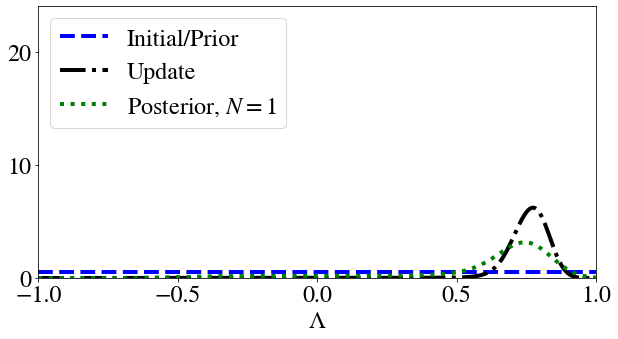
\includegraphics[width=0.49\linewidth]{figures/bip-vs-sip-1.png}
   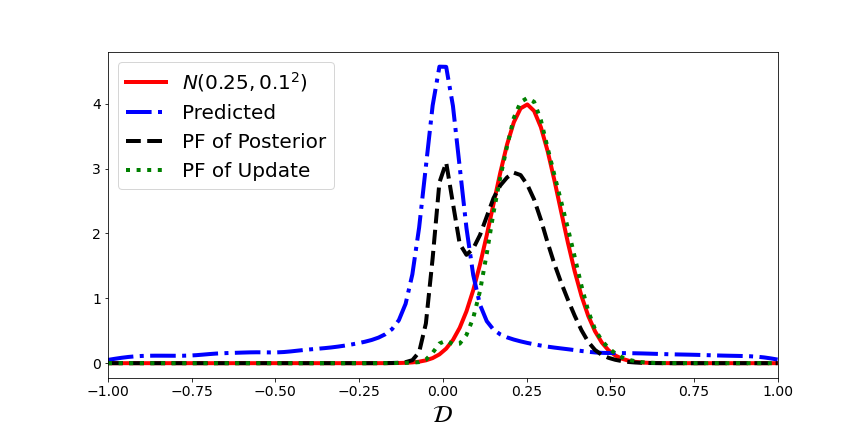
\includegraphics[width=0.49\linewidth]{figures/bip-vs-sip-pf-1.png}
 \caption{(Left) The initial/prior PDF $\initial$ (blue solid curve), updated PDF $\updated$ (black dashed curve), and posterior PDF $\pi_\text{post}$ (green dashed-dotted curve) on $\Lambda$.
 (Right) The push-forward (PF) of the initial/prior PDF $\predicted$ (blue solid curve), observed/likelihood PDF (red solid curve), PF of the updated PDF $\updated$ (black dashed curve), and the PF of the posterior PDF $\pi_\text{post}$ (green dashed-dotted curve) for the QoI.}
 \label{fig:bayes-comparison}
\end{figure}


While the updated and posterior densities in Fig.~\ref{fig:bayes-comparison} share certain similarities (e.g., they are uni-modal with similar locations of the mode), they are otherwise visibly distinct.
The differences between these densities is made more evident by examining their push-forwards.
The push-forward of the updated density agrees well with the observed density, which is to be expected.
However, the push-forward of the posterior is bi-modal and does not match the observed density, which we recall is identical to the data-likelihood function in this case.
%with peaks that appear to align fairly well with the two distinct peaks of the predicted density and observed density.
%Recall that the observed density and data-likelihood are, in this case, identical.
%Moreover, with the setup described above, the predicted density can also be interpreted as the push-forward of the prior density.
%This demonstrates the regularizing impact of the prior on the posterior and how i.

%
%Hierarchical Bayesian methods \cite{} extend this typical framework to problems where aleatoric uncertainties are present, but are still fundamentally developed from a  point estimation perspective.
%Specifically, prior distributions are specified from a parametric family of distributions, such as Gaussian distributions, and the hyper-parameters used to define that family of distributions, such as the means and variances, become a focal point of estimation by the methodology.

\end{ex}

The takeaway to the above discussion and example is that each density is solving a {\em different} inverse problem.
The posterior density is intended to provide point estimates of a true parameter value whereas the updated density is intended to quantitatively characterize natural variations in parameter values.
We reformulate the previous example to make the role of data collection more central in the follow example.

\begin{ex}
For the (Bayesian) Deterministic Inverse Problem, suppose $Q(\paramref)=0.25$ and noisy measurement data are drawn from a $N(0.25,0.1^2)$, i.e., we assume that each datum is given by $d=Q(\paramref)+\xi$ where $\xi\sim N(0,0.1^2)$.
For the SIP, we use the sample mean and variance of data to estimate the ``exact'' observed $N(0.25,0.1^2)$ distribution.
The observed density and data-likelihood are significantly different from one another, especially as more data are collected.
The data-likelihood is given by a product of normal densities.

We draw $M=5, 10, \text{ and}, 20$ samples to form estimates of $\observed$ and the likelihood functions.
We show the results in Figure~\ref{fig:bayes-comparison-convergence}.

\begin{figure}[htbp]
\centering
   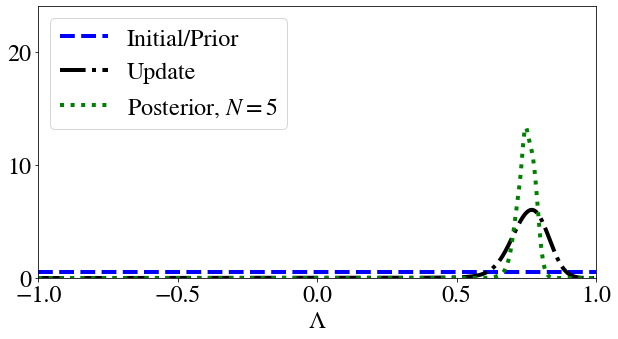
\includegraphics[width=0.49\linewidth]{figures/bip-vs-sip-5.png}
   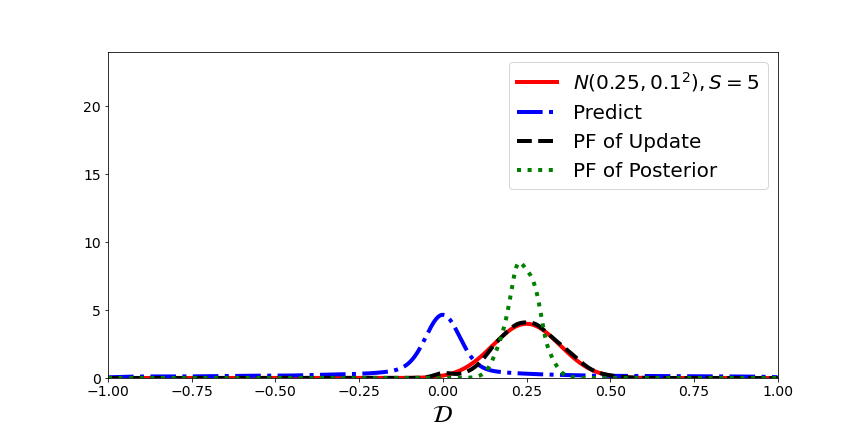
\includegraphics[width=0.49\linewidth]{figures/bip-vs-sip-pf-5.png}
   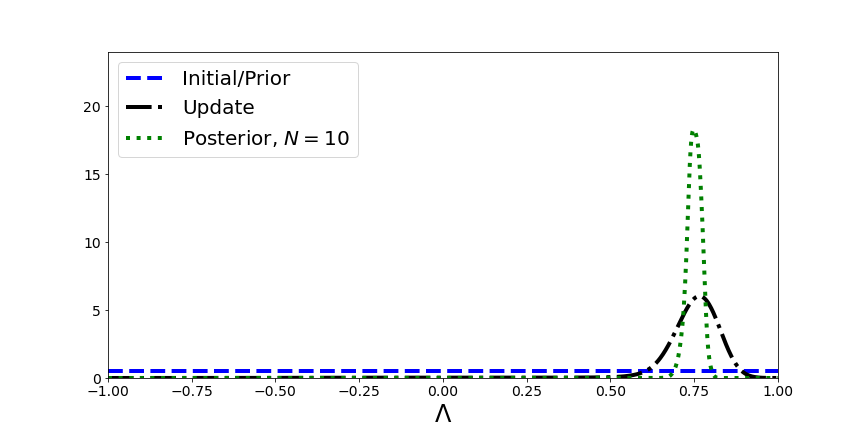
\includegraphics[width=0.49\linewidth]{figures/bip-vs-sip-10.png}
   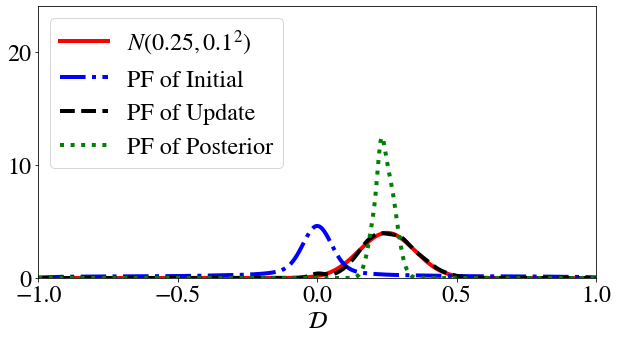
\includegraphics[width=0.49\linewidth]{figures/bip-vs-sip-pf-10.png}
   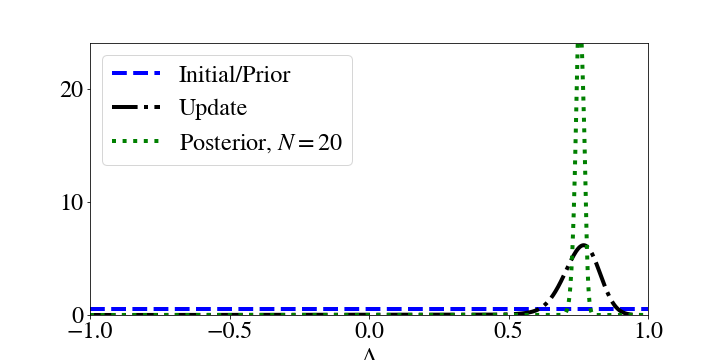
\includegraphics[width=0.49\linewidth]{figures/bip-vs-sip-20.png}
   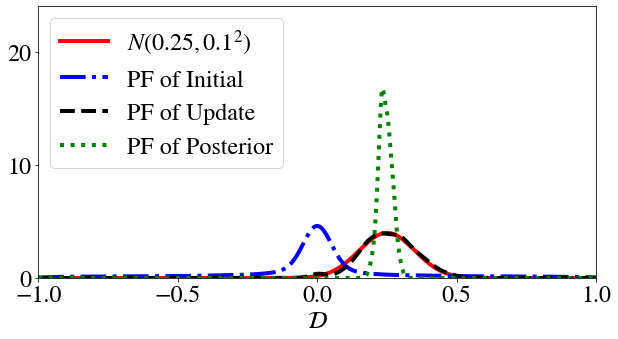
\includegraphics[width=0.49\linewidth]{figures/bip-vs-sip-pf-20.png}
 \caption{(Top to Bottom): $S=5, 10, \text{ and}, 20$ samples are used to solve the SIP and DIP for comparison. (Left) The initial/prior PDF $\initial$ (blue solid curve), updated PDF $\updated$ (black dashed curve), and posterior PDF $\pi_\text{post}$ (green dashed-dotted curve) on $\Lambda$.
 (Right) The push-forward (PF) of the initial/prior PDF $\predicted$ (blue solid curve), observed/likelihood PDF (red solid curve), PF of the updated PDF $\updated$ (black dashed curve), and the PF of the posterior PDF $\pi_\text{post}$ (green dashed-dotted curve) for the QoI.}
 \label{fig:bayes-comparison-convergence}
\end{figure}

For all values of $M$, the push-forward of the initial remains the same, and the push-forward of the update matches the observed.
By contrast, the posterior increases in confidence alongside the predictions it produces.
This further illustrates the point made earlier: the DIP and SIP are solving fundamentally different problems (they are addressing different questions).
The mean of the updated density could be used as an estimator to address the parameter identification problem, but collecting more data does not improve confidence.
As more data is incorporated, the goal of the DIP is to reduce epistemic uncertainty; for the SIP, it is to quantify the aleotoric uncertainty.

\end{ex}




%%%%%

In summary, it is not the goal of Bayesian inference to construct a pullback distribution.
Bayesian inverse problems are fundamentally posed as parameter-identification, not distribution estimation.
However, one could assume that a posterior on $\pspace$ can be expressed as a Gaussian distribution, and solve for the most likely mean and standard deviation that characterizes it [TK - cite more] \cite{Smith}.
This defines what is commonly referred to a as a Hierarchical Bayesian Inverse Problem.
More complex densities can be approximated by mixture models.

For example, one can assume that the posterior can be given by a linear combination of four Gaussian distributions, and solve for eight parameter values (four standard deviations and means).
However, the operative word here is \emph{assume}; in order to capture a density using a Bayesian framework, one needs to impose some sort of explicit structure on the posterior.
No such compromise is required in the DCI framework.
Distributions (or measures) can be solved for directly, regardless of any nonlinear/non-parameteric structure by leveraging the measure-theoretic approach described in \cite{BE13} or \cite{BJW18}.

It is important to note that Hierarchical Bayesian inverse problem casts a distribution-estimation problem in the context of parameter identification.
As a complementary line of reasoning, we seek to formulate a parameter identification problem in a DCI framework.
We revisit the results with a focus on parameter estimation using $\updated$. [TK - not sure what Troy's comment here means]

In Chapter~\ref{chapter:mud}, we motivate the use of the maximal updated density point (maximizing the update), as a means of providing a useful point estimate to parameters.
Before we proceed, we finish presenting some summarizing key results about the stability and numerical convergence of the updated solution \eqref{eq:updated-pdf} in the next section.

\FloatBarrier

\section{Properties and Assumptions of Consistent Update}\label{sec:properties}
Recall that the SIP is defined as finding a measure $\PP_\pspace$ such that the push-forward of it matched $\observedP$.
The following assumption guarantees the existence of a solution to the SIP in the form of an update to the initial distribution.
It implies that any event which is assigned a positive probability by the observations must also have a positive predicted probability.

\begin{assumption}[Predictability Assumption (Theoretical Form)]\label{as:predicted-theoretical}
  The measure associated with $\observed$ is absolutely continuous with respect to the measure associated with $\observed$.
\end{assumption}

If this is unsatisfied, one source of information (the data) suggests certain events are probable while another source of information (the model and initial beliefs) have a priori ruled that almost surely these events should not occur.
Therefore, either initial beliefs, the model under consideration, or the description of uncertainty encoded in $\predicted$ should be subjected to a critical reevaluation.

The following establishes a more practical form (from the perspective of numerical implementation), of \ref{as:predicted-theoretical} which states that the predicted measure must dominate the observed.
\begin{assumption}[Predictability Assumption (Practical Form)]\label{as:predicted-practical}
The requirement given in Assumption~\ref{as:predicted-theoretical} is guaranteed if the following is satisfied:
\begin{equation}\label{eq:pred-pract}
  \exists \; C>0 \text{ such that } \observed (\q) \leq C \predicted(\q) \text{ for a.e. } d\in \dspace,
\end{equation}
where it is understood that $\q = \qlam$ for some $\param \in \pspace$.
\end{assumption}

Assumption~\ref{as:predicted-practical} is particularly useful in that it is the same condition required for applying rejection sampling, which we summarize in Algorithm~\ref{alg:rejection}.
Specifically, this allows us to sample from the updated density using the initial density as follows:

\begin{algorithm}[hbtp]
\DontPrintSemicolon
Draw $\nsamps$ independent identically distributed (i.i.d.) initial samples from the initial density
	\For{$\iparam = 1, \hdots, \nsamps$}{
	    Compute $\Qi = \qoi(\param^{(\iparam)})$.\\
	}
	Approximate $\predicted$, the push-forward of $\initial$, by some method such as kernel density estimation.
  \For{$\iparam = 1, \hdots, \nsamps$}{
	    Compute $r\lami = \frac{\observed\Qi}{\predicted\Qi}$.\\
	}
  Normalize $r$ by dividing it by $\max(r)$.
  \For{$\iparam = 1, \hdots, \nsamps$}{
      Draw a sample from a standard uniform distribution.
	    If the value of $r\lami$ exceeds the value of the random sample, keep $r\lami$.\\
	}
 \caption{Rejection Sampling Leveraging Ratio from Density-Based Approach}
 \label{alg:rejection}
\end{algorithm}

Now, assuming \eqref{eq:pred-pract} holds, we state the following theorem from \cite{BJW18a} based upon the disintegration of measures:

\begin{thm}[Existence and Uniqueness]
  For any set $A\in \pborel$, the probability measure $\updatedP$ defined by
  \begin{equation}\label{eq:dci_sol}
    \updatedP (A) = \int_\dspace \left (  \int_{\pspace \in \qoi^{-1}(\q)}  \initial\lam \frac{\observed\Q}{\predicted\Q} \, d\mu_{\pspace, \q} \lam \right ) \, d\dmeas(\q), \; \forall \; A \in \pborel
  \end{equation}
  is a consistent solution to the SIP given in (\ref{eq:inverse-problem}), and is uniquely defined up to the specification of the initial probability measure $\initial$ on $(\pspace, \pborel)$.
  Here, $\mu_{\pspace, d}$ denotes the disintegration of the dominating measure $\mu_\pspace$.
\end{thm}

The updated density \eqref{eq:update} in the iterated integral in \eqref{eq:dci_sol} has no normalization constant because it is in fact a density (i.e., it integrates to $1$), which is summarized in Corollary 3.1 in \cite{BJW18a} and restated in simplified form below:
\begin{cor}\label{cor:int}
$\updatedP(\pspace) = 1$.
\end{cor}

These definitions are combined to identify the form of the \emph{updated density}, originally derived in \cite{BJW18a}:

\begin{defn}[Updated Distribution]\label{defn:updated}
  A solution satisfying \eqref{eq:dci_sol} is referred to as an updated distribution, with an updated density
  \begin{equation}\label{eq:update}
    \updated \lam = \initial \lam \frac{\observed \Q }{\predicted \Q }, \; \forall \; \param \in \pspace.
  \end{equation}
\end{defn}

% Corollary~\ref{cor:int} is critical to understanding some significant differences between the classical Bayesian posterior density~\cite{Smith} and the updated density density given by \eqref{eq:update}, which we discuss in Section~\ref{sec:othermethods} as well as other places throughout this thesis.
% Moreover, this Corollary provides the basis for a useful numerical diagnostic that assesses both the quality of a numerical approximation of $\updated$ based on finite sampling and density estimation as well as any potential violations of the predictability assumption.

% We next turn our attention to attributes of the Data-Consistent framework which make it appealing for use in solving inverse problems.
% Namely, we summarize the stability results first presented in \cite{BJW18} that demonstrate that approximation errors in the updated density are well understood within the measure-theoretic foundation on which the approach is constructed.

%%%%%%%%%%%%%%%%%%%%%%%%

\subsection{Stability of the Consistent Solution}\label{sec:stability}
The Total Variation (TV) metric on a space of probability measures, absolutely continuous with respect to a dominating measure $\mu$, is defined as
\begin{equation}\label{eq:tv}
d_{\text{TV}} (\PP_f, \PP_g) := \int \abs{\pp_f - \pp_g} \, d\mu,
\end{equation}
where $\pp_f,\pp_g$ are the densities (Radon-Nikodym derivatives with respect to $\mu$), associated with measures $\PP_f, \PP_g$, respectively.
The stability results below are all with respect to the TV metric, which is widely used in the literature and is also known as \emph{statistical distance}~\citep{GS02, Smith, Silverman}.
We first define stability with respect to perturbations in the data.

\begin{defn}[Stability of Updated Densities I]\label{defn:stableobs}
  Given $\initialP$ and $\observedP$, let $\widehat{\observedP}$ be any perturbation to $\observedP$ on $(\dspace, \dborel)$ satisfying \eqref{eq:pred-pract}.
  Let $\updatedP$ and $\widehat{\updatedP}$ denote the consistent solutions associated with $\observedP$ and $\widehat{\observedP}$, respectively.
  We say that $\updatedP$ is \emph{stable} with respect to perturbations in $\observedP$ if for all $\eps > 0$, there exists a $\delta > 0$ such that
  \begin{equation}
    d_{\text{TV}} (\observedP, \widehat{\observedP}) < \delta \implies d_{\text{TV}} (\updatedP, \widehat{\updatedP}) < \eps.
  \end{equation}
\end{defn}

In \cite{BJW18a}, it is shown that $d_{\text{TV}} (\widehat{\updatedP}, \updatedP) = d_{\text{TV}} (\widehat{\observedP}, \observedP)$, which immediately proves the following:

\begin{thm}
  $\updatedP$ is stable with respect to perturbations to $\observedP$.
  \label{thm:stableobs}
\end{thm}

This next definition and result are useful in analyzing the sensitivity of the updated density with respect to the initial beliefs.

\begin{defn}[Stability of Updated Densities II]\label{defn:stableinitial}
  Given $\initialP$ and $\observedP$, let $\widehat{\initialP}$ be any perturbation to $\initialP$ on $(\pspace, \pborel)$ satisfying \eqref{eq:pred-pract}.
  Let $\updatedP$ and $\widehat{\updatedP}$ denote the consistent solutions associated with $\observedP$ and $\widehat{\observedP}$, respectively.
  Let $\sett{\PP_{\pspace, d}}{d\in\dspace}{}$ and $\sett{\widehat{\PP_{\pspace, d}}}{d\in\dspace}{}$ be the conditional probabilities defined by the disintegration of $\initialP$ and $\widehat{\initialP}$, respectively.
  We say that $\updatedP$ is \emph{stable} with respect to perturbations in $\initialP$ if for all $\eps > 0$, there exists a $\delta > 0$ such that for almost every $d\in\supp(\observedP)$,
  \begin{equation}\label{eq:stableinitial}
    d_{\text{TV}} (\PP_{\pspace, d}, \widehat{\PP_{\pspace, d}}) < \delta \implies d_{\text{TV}} (\updatedP, \widehat{\updatedP}) < \eps.
  \end{equation}
\end{defn}

The following important stability theorem is also proven in \cite{BJW18a}:

\begin{thm}
  $\updatedP$ is stable with respect to perturbations to $\initialP$
  \label{thm:stableinitial}
\end{thm}

Taken together, these stability results provide assurance that the updated density we obtain is accurate up to the level of experimental error polluting $\observedP$ and error in incorrectly specifying initial assumptions using $\initialP$.
Given that specifying the definition of a ``true'' initial density is somewhat nebulous, we are less interested in the consequences of the latter conclusion.
However, generating samples from $\updatedP$ generally requires a numerical approximation to the predicted distribution, which introduces additional errors in $\updatedP$.
In Section~\ref{sec:approx}, the TV metric is used to bound the error in the updated density in terms of the error in the approximation to the push-forward of the initial.




%%%%%%%%% Section 2.3
\subsection{Numerical Approximation and Sampling}\label{sec:approx}
%Since we are given $\initial$ and $\observed$, the computation of $\predicted$ is the only aspect of the Consistent Bayesian framework that needs to be approximated.
%Since there are few restrictions on the structure of the map $\qoi$ that defines $\predicted$, there is in general no explicit expression from which we can generate samples, so we use a numerical approximation to the probability density function.
%
%For simplicity, we simply propagate Monte-Carlo samples from the prior and use a kernel density estimate (usually Gaussian\footnote{In this proposal, all results are generated using this kernel, though six kernels common to density estimation are implemented in the ConsistentBayes Python package [TK - cite Silverman and your github].}).
%
%We summarize this in the following algorithm:
%
%\begin{algorithm}[hbtp]
%\DontPrintSemicolon
%Generate a set of samples $\sett{\param_i}{i=1}{N}$
%	\For{$i = 1, \hdots, N$}{
%			Propagate sample $\param_i$ through the QoI map. Set $d_i = \qoi(\param_i)$.
%	}
%Use $\sett{d_i}{i=1}{N}$ and a density estimation method to approximate $\predicted$.
%	\label{alg:sample}
%\caption{Numerical Approximation of the Push-forward of the Prior Density}
%\end{algorithm}
%


%The computational object associated with $\predicted$ is stored for re-use and can be evaluated at locations in $\dspace$ other than $\sett{d_i}{i=1}{N}$.
%This procedure should be thought of as a characterization of the data space given the prior assumptions encoded in $\initial$.

If $\widehat{\predicted}$ denotes a computational approximation to the push-forward of the initial density obtained with $\widehat{\predicted}$ substituted for $\predicted$ in \eqref{eq:dci_sol}, then the conditional densities from the Disintegration Theorem (c.f. Chapter~\ref{chapter:geometry} for more details), are given as
\[
\frac{\widehat{d\PP_{\pspace, d}}}{d\mu_{\pspace, d}\lam} = \frac{\initial\lam}{ \widehat{\predicted\Q} },
\]
where $\widehat{\PP_{\pspace, d}}$ denotes the disintegration of $\widehat{\updatedP}$.


We assume the following for the approximation of the push-forward of the initial density:
\begin{assumption}\label{as:predicted-theoreticalx}
There exists some $C>0$ such that
\[
\observed (d) \leq C \widehat{\predicted(d)} \text{ for a.e. } d\in \dspace.
\]
\end{assumption}

If this assumption is satisfied, then from \cite{BJW18a}, we have the following:
\begin{thm}\label{thm:predicted_bound}
  The error in the approximate updated density is bounded above:
  \begin{equation}\label{eq:predicted_bound}
    d_{\text{TV}} (\updatedP, \widehat{\updatedP}) \leq C d_{\text{TV}} (\predictedP, \widehat{\predictedP}),
  \end{equation}
  where the $C$ is the constant taken from Assumption \ref{as:predicted-theoreticalx}.
\end{thm}

A straightforward approach to construct $\widehat{\predicted}$ is to use a forward propagation of samples from $\pspace$ to $\dspace$ and then apply kernel density estimation (KDE)~\citep{BJW18a}.
Then, we may evaluate $\updated$ directly for any sample of $\pspace$ at the cost of one model solve per sample.
While this allows us to incorporate sophisticated sampling techniques such as Markov-Chain Monte-Carlo (MCMC)~\citep{Smith, Tarantola_book} to generate samples according to the updated distribution, we often opt for a simpler route based on rejection sampling by re-using the initial set of propagated samples.
This avoids any additional model evaluations (as would be required by techniques relying on proposal samples such as MCMC).
We leverage the re-use of samples in the results herein extensively.

By Theorem~\ref{thm:predicted_bound}, the accuracy of the computed updated density relies on the accuracy of the approximation of the push-forward of the initial.
Throughout this thesis, we utilize a KDE with a Gaussian kernel to produce the non-parametric estimates of $\predicted$.
Such KDEs are known to converge at a rate of $\mathcal{O}(N^{-4/(4+\dimD)})$ in mean-squared error and $\mathcal{O}(N^{-2/(4+\dimD)})$ in $L^1$-error, where $\dimD$ is the dimension of $\dspace$, and $N$ is the number of samples from $\initial$ propagated through $\qoi$ \citep{Silverman}.

For simplicity, we introduce the following notation to capture the role of the ratio involved in \eqref{eq:dci_sol} to demonstrate properties we can leverage for generating samples from $\updated$.
We let
\[
\updated\lam = \initial \lam r\Q, \text{ where } r\Q = \frac{\observed\Q}{\predicted\Q}.
\]

Many standard calculations about the updated density involve integrals of functions of $r\Q$ with respect to the prior.
For any measurable function $f$, we establish the connection of calculating quantities over $\pspace$ with those over $\dspace$ by leveraging the following identity:
\[
\int_\pspace f\left( r\Q \right ) \, d\initialP = \int_\dspace f\left( r(\q) \right ) \, d\predictedP
\]

We use several throughout this thesis, including the integral of the updated density:
\[
I(\updated ) = \int_\pspace r\Q \, d\initialP = \int_\dspace r(\q) \, d\predictedP ,
\]
which we can use to validate that $I(\updated) = 1$ in order to numerically validate that the predictability assumption given in \eqref{eq:predicted_bound} was not violated.
The sample average of $r(\q)$ can be used to estimate $I(\updated)$.
This convenience is afforded by the fact that the i.i.d. samples provide us with the ability to take a Monte-Carlo estimate of the integral.

% Similarly, we follow \cite{BJW18} to write the commonly used metric for Information Gain, the Kullback-Liebler (KL) divergence:
% \begin{equation}\label{eq:KLdiv}
% \text{KL}(\initial : \updated ) = \int_\pspace r\Q \log r\Q \, d\initialP = \text{KL}(\observed : \predicted ),
% \end{equation}
% i.e., the KL-divergence between the initial and updated density is equal to the KL-divergence between the observed and the predicted densities.

Taken together, the results summarized in this section demonstrate that the Data-Consistent framework and density-based solution \eqref{eq:dci_sol} have been rigorously constructed and studied.
They give an experimenter assurance that there are not unexpected consequences for small mistakes in problem formulation.
In the following section, we provide a similar sense of assurance for a central practical consideration involved in this work: that the results depend on computational implementations of the aforementioned theory, i.e., software.
We directly address how to establish a complementary level of rigor to the implementation of the work as was invested in the construction of the theory.
We leverage modern advances in software engineering with an emphasis on results being reproducible in an accessible manner.

\section{Towards a Reproducible Thesis}\label{sec:reproducibility}

\subsection{Motivations}\label{sec:motivations}
In some respects, the practice of writing software has diverged from the motivations of an academic researcher.
The latter seeks to generate new knowledge and may write a set of example scripts/programs to demonstrate some novel idea or method.
By contrast, the motivations of a software engineer are related to resiliency.
Not only must they ensure the code works as expected given a myriad of ways users may interact with it, but it is necessary to write the code in a manner compatible with maintaining it into the future.
Much of the work of writing ``good software'' is concerned with writing appropriate documentation to express the intended usage and logic underlying architectural decisions.
There are many ways to write a functioning program to demonstrate a proof-of-concept, but creating something that is \emph{user-friendly}, guaranteed to be free of mistakes, and scales across different computational environments/resources requires an entirely different approach.

Decisions made early in the software design cycle have lasting impacts on future features and functionality.
Rigor is added to libraries through the writing of \emph{unit tests}, and use of \emph{continous integration} ensures that the download and installation process is predictable and reproducible.
Code that only runs on the author's computer is impractical, since any thorough critique requires independent verification.
Without proper context and architecture, new ideas that are implemented in programs are unlikely to be adopted.


This thesis is concerned not only with a demonstration of novel mathematical content\---showcasing new ways to make inferences from noisy data in a novel Data-Consistent framework\---it also serves to document the process of ensuring that the work is \textbf{fully reproducible}.
In mathematics, reproducibility is ensured through the use of proofs, which motivate the original work presented here.
However, as the title of this thesis suggests, much of the focus is actually on the computational implementation of the novel research into Data Consistent Inversion, studying the impact of using computers to perform the task of making conclusions based on data.
Mathematics is implemented on computers through software.
We are therefore concerned with ensuring the expected functionality of that software, which aligns with our training as mathematicians; we care deeply about making sure things are rigorous.

In short, we want to make sure that theory aligns with practice, and that both live up to high standards of intellectual scrutiny.
Every computational result, illustrative figure, table, plot, etc. presented in this thesis is associated with the scripts that generate them, and are included in the  repository for this document [TK - cite].
It is written in \LaTeX~(which is itself a programming language), and presents its own software dependencies in addition to those required to run the scripts to generate the images and tables.
To address this concern, we leverage \emph{Travis}, a continuous integration service [TK-cite], to ensure that all figures can be generated and the \LaTeX\, document compiles into a PDF.

The same care is taken to ensure the reproducibility of all numerical results based on software.
An \emph{image} that contains a fully pre-built Linux software environment within which one can compile the thesis and run the code is available through the Docker Cloud registry [TK -cite].
The latter enables the ability to generate this thesis document in its entirety on any software platform that supports Docker (Windows, MacOS, Linux).
A cloud service called Binder [ TK - cite mybinder.org] allows one-click deployments in any web-browser, removing the need for any installation whatsoever for anyone wanting to reproduce the contents of this document.




%%%%%%%%%%%%%%%%%%%%%%%%%%%%%%%%%%%%%%%%%%%%%%%%%%
\section{Outline of Remaining Chapters}\label{sec:outline}
In Chapter~\ref{chapter:mud}, we propose a way by which parameter identification can be performed in the DCI framework by posing the problem as a SIP and maximizing $\updated$.
Central to how this contribution is accomplished in practice is the definition of a data-constructed QoI map.
The impact of a QoI's inherent geometric properties on our ability to approximate solutions to SIPs using finite sampling is then summarized in Chapter~\ref{chapter:geometry}.
The focus there is on the property called skewness, which is connected to the QoI maps introduced in \ref{chapter:mud} through a case study of a PDE-based example in Chapter~\ref{chapter:vector-valued}.
Finally, we provide some concluding remarks and directions for future research in Chapter~\ref{chapter:future} alongside several examples demonstrating preliminary results for novel extensions of the work presented in this thesis.

